\section{Protégé}
\label{sec:protege}

Protégé\footnote{\url{https://protege.stanford.edu/}} is the most popular free and open source\footnote{\url{https://github.com/protegeproject/protege}} ontology development environment.\footnote{\url{https://protege.stanford.edu/shortcourse/}} The first version was developed by Mark Musen in 1987, and has been so far by a team at Stanford University \cite{gennari2003evolution}. The latest version, 5.5.0, has been released in March 2019. In recent years, in addition to the desktop version, a web version, called WebProtégé\footnote{\url{https://webprotege.stanford.edu/}} is also being developed, focused on collaborative viewing and editing.

Protégé supports creation and editing of one or more ontologies, providing a customizable graphic user interface. Among the several features available in Protégé, the most relevant are the possibility to create, rename and delete entities, add notations, merge ontologies, and more. It also includes a visualization tool for interactive navigation of ontology relationships and different reasoners.

The two most important sections for creating and editing an ontology are the "Active ontology" and "Entities" tabs. The first, that is opened by default, is designed to view and edit the information of the ontology, such as its \ac{IRI}, its annotations and the imported ontologies. On the right there is also a panel that reports some metrics about the ontology, such as the total number of axioms, classes, properties, and more. Figure \ref{fig:protege-home} shows an example of the "Active ontology" tab.

\begin{figure}[!ht]
  \centering
  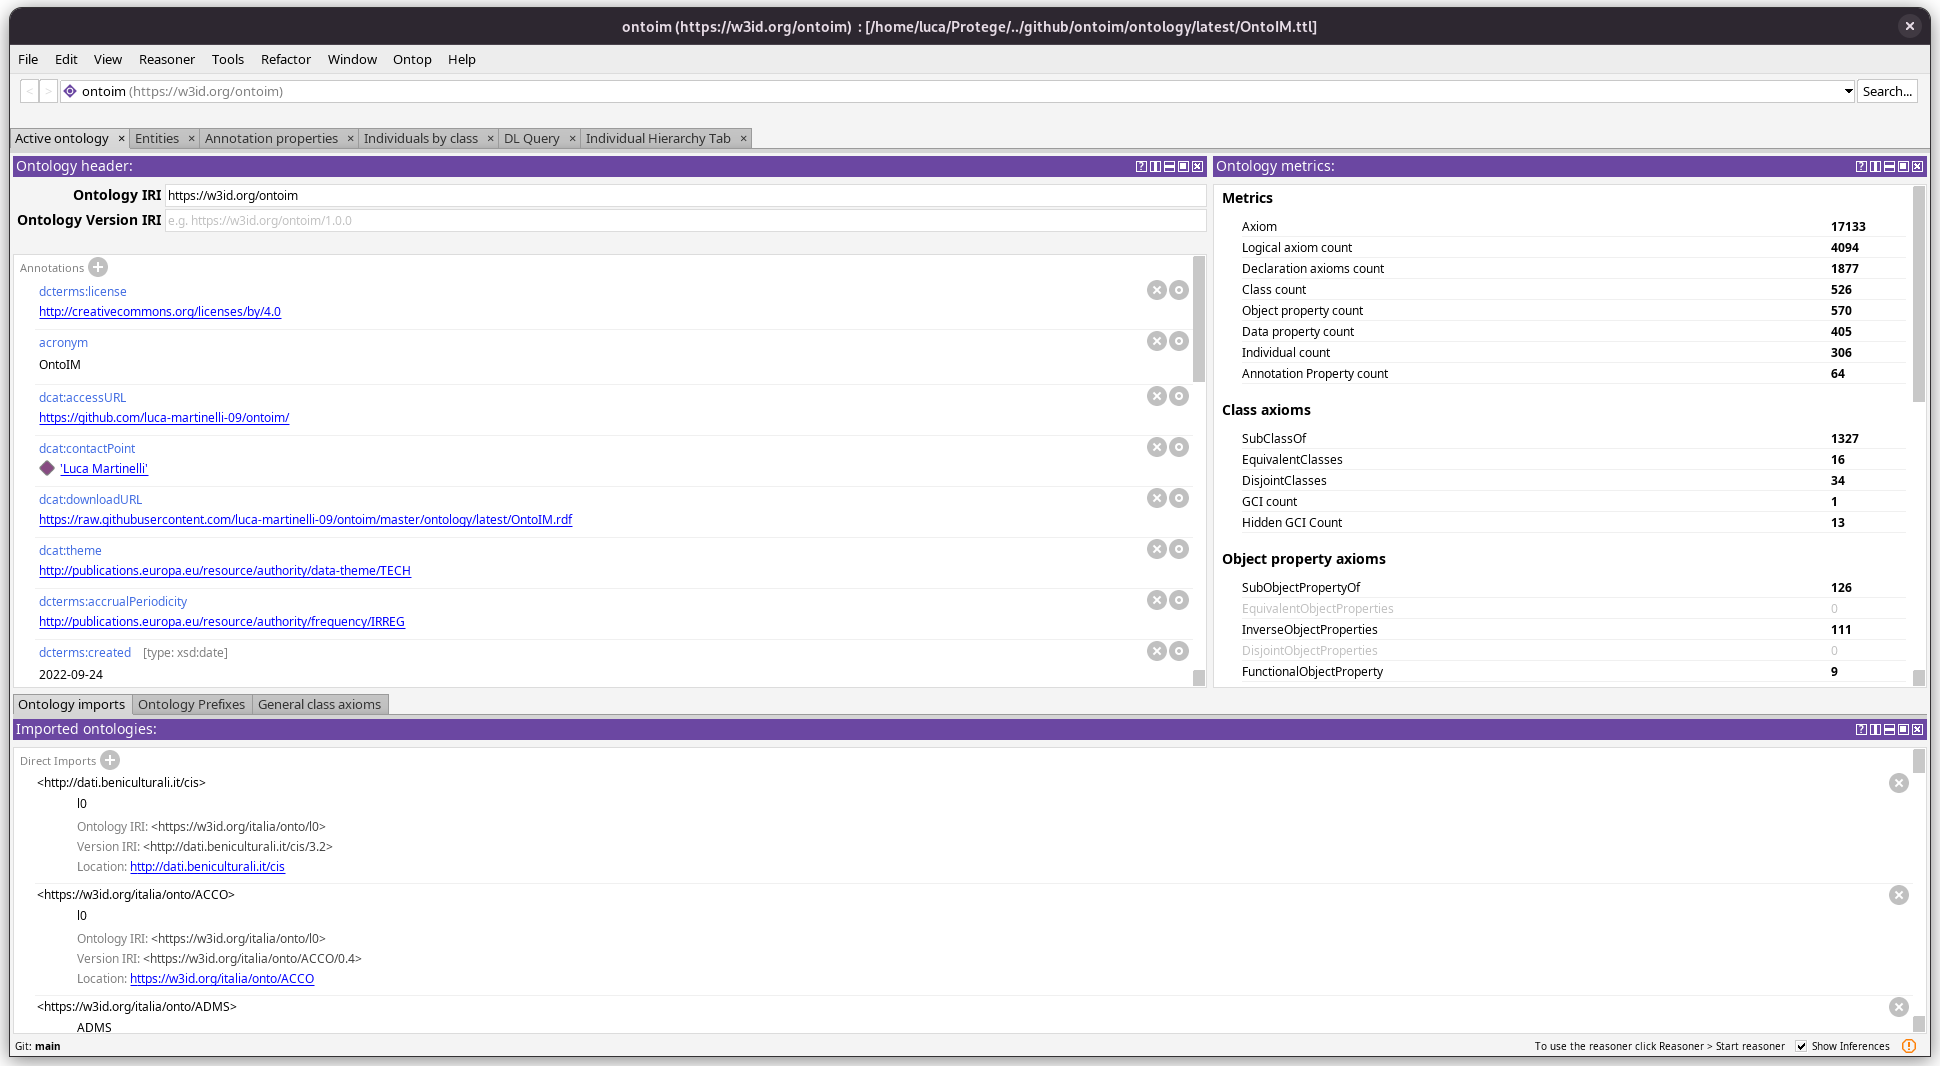
\includegraphics[width=\columnwidth]{images/protege/protege-home}
  \caption{A snapshot of the Protégé "Active ontology" tab.}
  \label{fig:protege-home}
\end{figure}

The "Entities" tab is the most important section for creating an ontology. Indeed, in this tab it is possible to manage the classes, the properties (object properties, data properties, and annotation properties), datatypes and individuals. The left part provides a navigation tool to select, add and deletes entities, while the right part is focused on viewing and editing the selected entity by adding properties and axioms. Figure \ref{fig:protege-entities} shows an example of the "Entities" tab.

\begin{figure}[!ht]
  \centering
  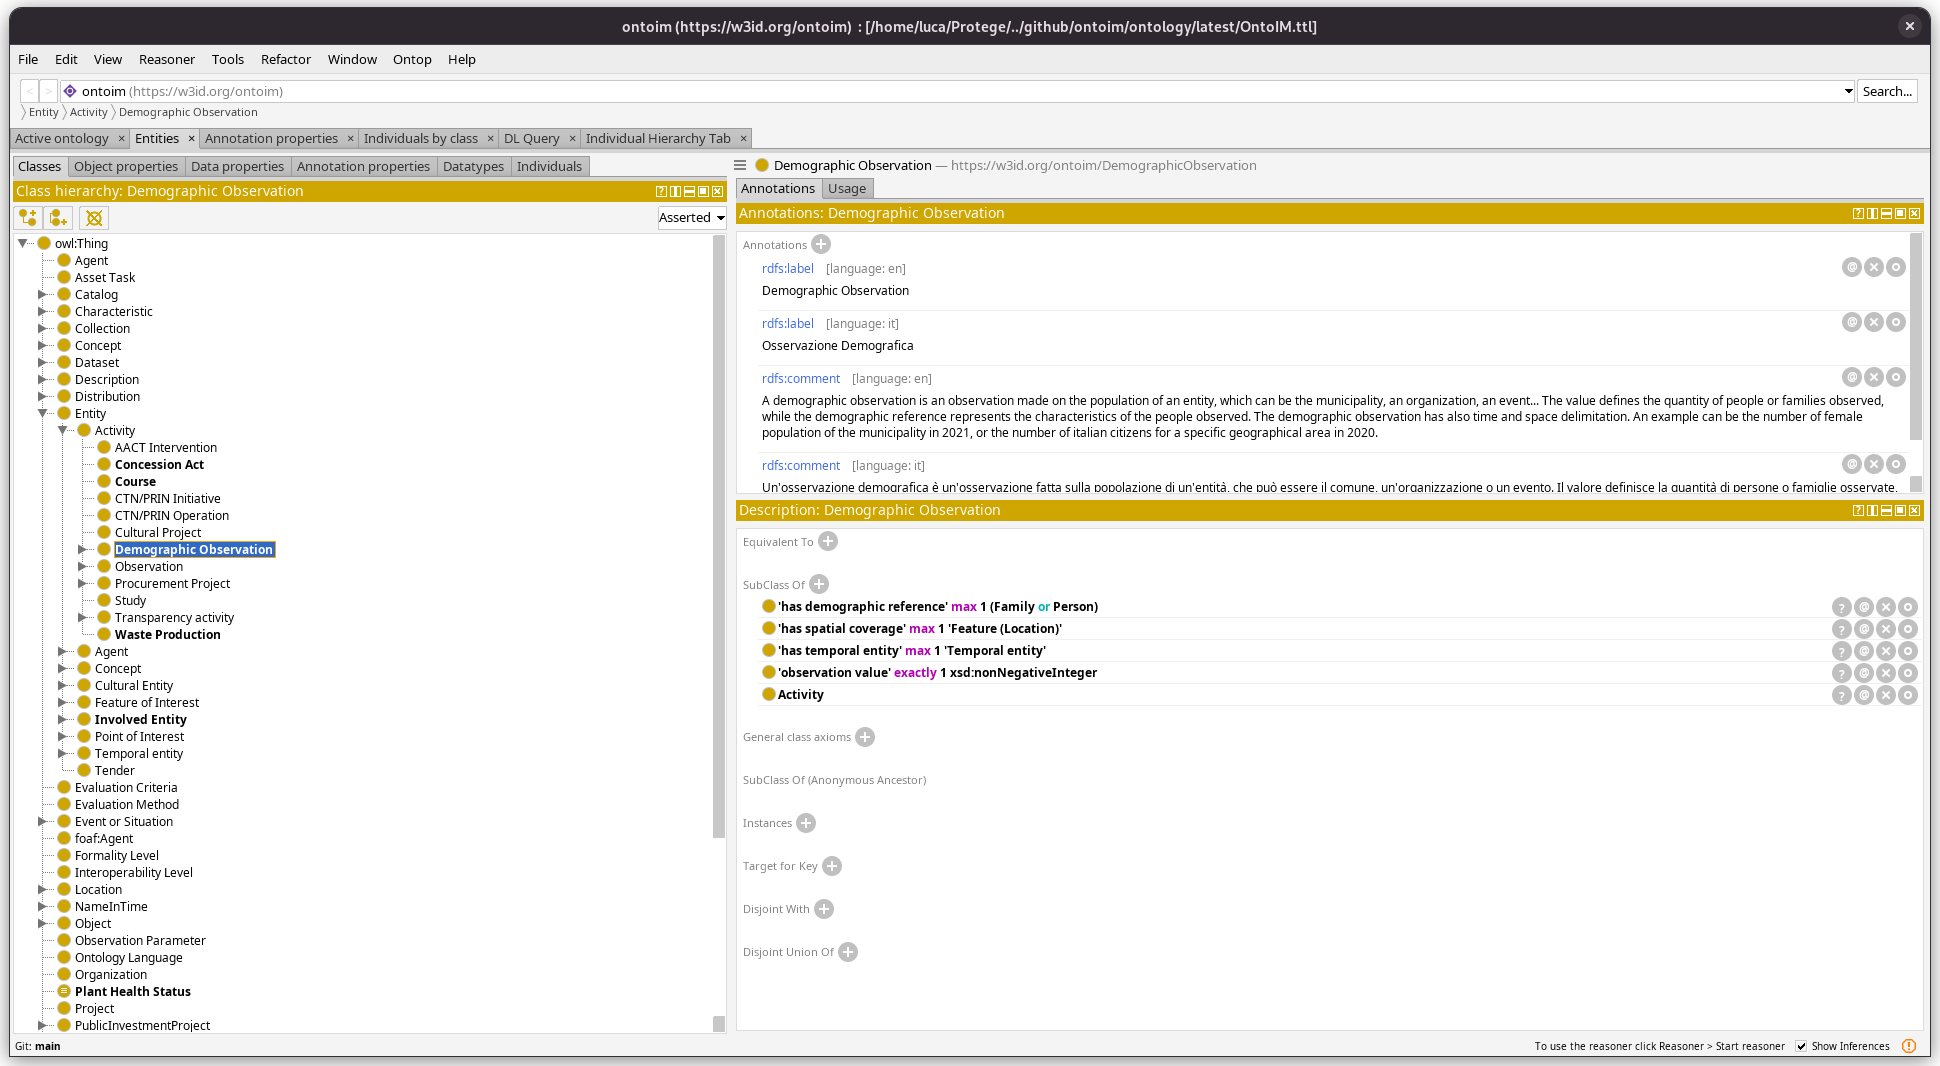
\includegraphics[width=\columnwidth]{images/protege/protege-entities}
  \caption{A snapshot of the Protégé "Entities" tab.}
  \label{fig:protege-entities}
\end{figure}